\chapter{ANÁLISE E MODELAGEM}

A primeira versão de arquitetura do projeto, será desenvolvida neste capítulo, além de
requisitos funcionais e não funcionais. Utilizarei o site "draw.io"para realizar os desenhos, fluxos
e primeira seção de arquitetura, além de exemplificar as regras da arquitetura. Nas próximas
versões do projeto, será utilizada tecnologia C4 model para exemplificar e desenhar os diagramas.

\section{Modelo Arquitetural}
Para o desenvolvimento do trabalho, utilizando modelos arquiteturais como micro ser-
viços e mensageria, será desenvolvido 5 micro serviços, todos escritos em NodeJs/NestJs e
Typescript. Para o API Gateway será desenvolvido uma aplicação em NodeJS. Como citado
anteriormente, o Gateway é o coração de uma aplicação baseada em micro serviços, para realizar
o roteamento entre eles.

Para banco de dados, será utilizado o MongoDB para salvar informações como logger
e usuários, já no Supabase, será salvo os documentos de cada usuário. Cada usuário terá uma
coleção de documentos. Foram escolhidas essas tecnologias para salvar os dados, pois são
utilizadas em larga escala em aplicações de micro serviços.

\begin{figure}[!ht]
    \centering
    \caption{Arquitetura da aplicação}
    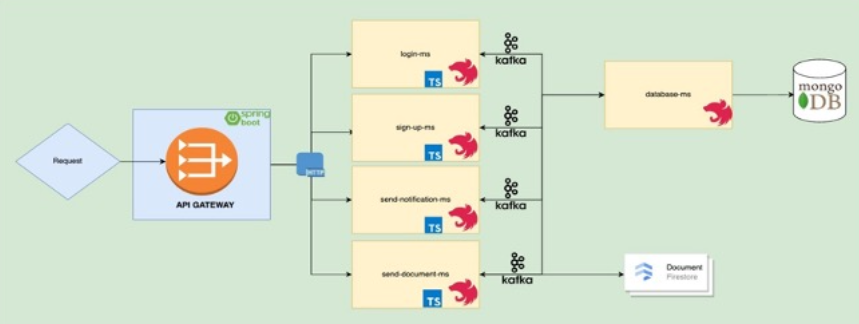
\includegraphics[scale=0.44]{assets/application-arch}
    \label{fig:application-arch}
    \tiny
    \sourcemedaddy
\end{figure}


\section{Requisitos funcionais e não funcionais}
